\let\negmedspace\undefined
\let\negthickspace\undefined
\documentclass[journal]{IEEEtran}
\usepackage[a5paper, margin=10mm, onecolumn]{geometry}
%\usepackage{lmodern} % Ensure lmodern is loaded for pdflatex
\usepackage{tfrupee} % Include tfrupee package

\setlength{\headheight}{1cm} % Set the height of the header box
\setlength{\headsep}{0mm}     % Set the distance between the header box and the top of the text

\usepackage{gvv-book}
\usepackage{gvv}
\usepackage{cite}
\usepackage{amsmath,amssymb,amsfonts,amsthm}
\usepackage{algorithmic}
\usepackage{graphicx}
\usepackage{textcomp}
\usepackage{xcolor}
\usepackage{txfonts}
\usepackage{listings}
\usepackage{enumitem}
\usepackage{mathtools}
\usepackage{gensymb}
\usepackage{comment}
\usepackage[breaklinks=true]{hyperref}
\usepackage{tkz-euclide} 
\usepackage{listings}
% \usepackage{gvv}                                        
\def\inputGnumericTable{}                                 
\usepackage[latin1]{inputenc}                                
\usepackage{color}                                            
\usepackage{array}                                            
\usepackage{longtable}                                       
\usepackage{calc}                                             
\usepackage{multirow}                                         
\usepackage{hhline}                                           
\usepackage{ifthen}                                           
\usepackage{lscape}
\usepackage{circuitikz}
\tikzstyle{block} = [rectangle, draw, fill=blue!20, 
    text width=4em, text centered, rounded corners, minimum height=3em]
\tikzstyle{sum} = [draw, fill=blue!10, circle, minimum size=1cm, node distance=1.5cm]
\tikzstyle{input} = [coordinate]
\tikzstyle{output} = [coordinate]


\begin{document}

\bibliographystyle{IEEEtran}
\vspace{3cm}

\title{2.7.11}
\author{AI25BTECH11039-Harichandana Varanasi}
 \maketitle
% \newpage
% \bigskip
{\let\newpage\relax\maketitle}

\renewcommand{\thefigure}{\theenumi}
\renewcommand{\thetable}{\theenumi}
\setlength{\intextsep}{10pt} % Space between text and floats


\numberwithin{equation}{enumi}
\numberwithin{figure}{enumi}
\renewcommand{\thetable}{\theenumi}



\date{}

\begin{document}
\maketitle


\section*{Question}
\textbf{Q 2.7.11.} Find the area of the triangle with vertices
$A=\myvec{1\\-1}$,\; $B=\myvec{-4\\6}$,\; $C=\myvec{-3\\-5}$.


\section*{Solution}
Let 
\vec{A} = \myvec{1\\-1},\;
\vec{B} = \myvec{-4\\6},\;
\vec{C} = \myvec{-3\\-5}.
 then
\[
\vec{m} = \vec{B} - \vec{A} = \myvec{-5\\7}, \quad
\vec{n} = \vec{C} - \vec{A} = \myvec{-4\\-4}.
\]
The area of the triangle is
\[
\Delta = \frac{1}{2}\,\abs{\det\myvec{\vec{m} & \vec{n}}}
= \frac{1}{2}\,\abs{(-5)(-4) - (7)(-4)}
= \frac{1}{2}\,(48) = \boxed{24}.
\]


   \begin{figure}[h!]
\centering
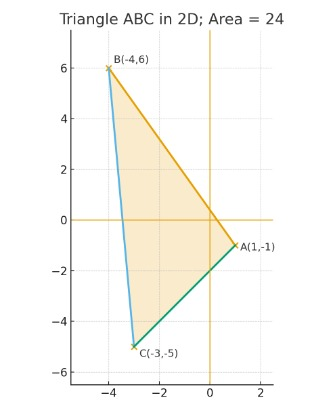
\includegraphics[width=0.7\linewidth]{figs/2.7.11.jpeg}
\caption{Triangle $ABC$ with $A(1,-1)$, $B(-4,6)$, $C(-3,-5)$; area $=24$.}

\end{figure} 

\end{document}
